\documentclass{article}
\usepackage{graphicx}
\usepackage{float}
\begin{document}

\title{Exchange Volume Shares} \author{Paul Kim and Teddy Cho}

\maketitle
\vspace{.5pc}

\section{Data for Macro Trends}
We use historical data from the NYSE Trade and Quote database\footnote{We note that this data is known to have inaccuracies regarding quotes' timestamps, and such issues may carry over to trade timestamps. These issues stem from timestamps originating from a secondary source (i.e., not the exchanges' order matching engines) and being derived after an exchange aggregation method which introduces further latency\footnote{See Budish, Cramton and Shim (2015) and Ding, Hanna and Hendershott (2014)}.}, made available by Wharton Research Data Services. The dataset ``contains intraday transactions data (trades and quotes) for all securities listed on the New York Stock Exchange (NYSE), American Stock Exchange (AMEX), as well as Nasdaq National Market System (NMS) and SmallCap issues''\footnote{See https://wrds-web.wharton.upenn.edu/wrds/ds/taq/index.cfm.}.\\

Our data cover all trades for a sample of symbols\footnote{Our sample of symbols consists of AMD, BAC, C, GOOG, GRPN, JBLU, MSFT, and RAD.} over the period of Mar 1, 2014 - Mar 31, 2014. No time filtering is used, and we are left with 20??? trading days total.\\

\section{Macro Trends}
\subsection{Daily Exchange Shares}
To get a sense of trends of where stocks trade, we compute the daily exchange shares for each stock $i$ on exchange $j$ for day $t$ from its trade volumes $q$\\
$$s_{ijt} = \frac{q_{ijt}}{q_{it}}.$$\\
This $s_{ijt}$ was plotted and stored in Dropbox under the /exchangeShare/ folder. A few are shown here:\\
\begin{figure}[H]
\centering
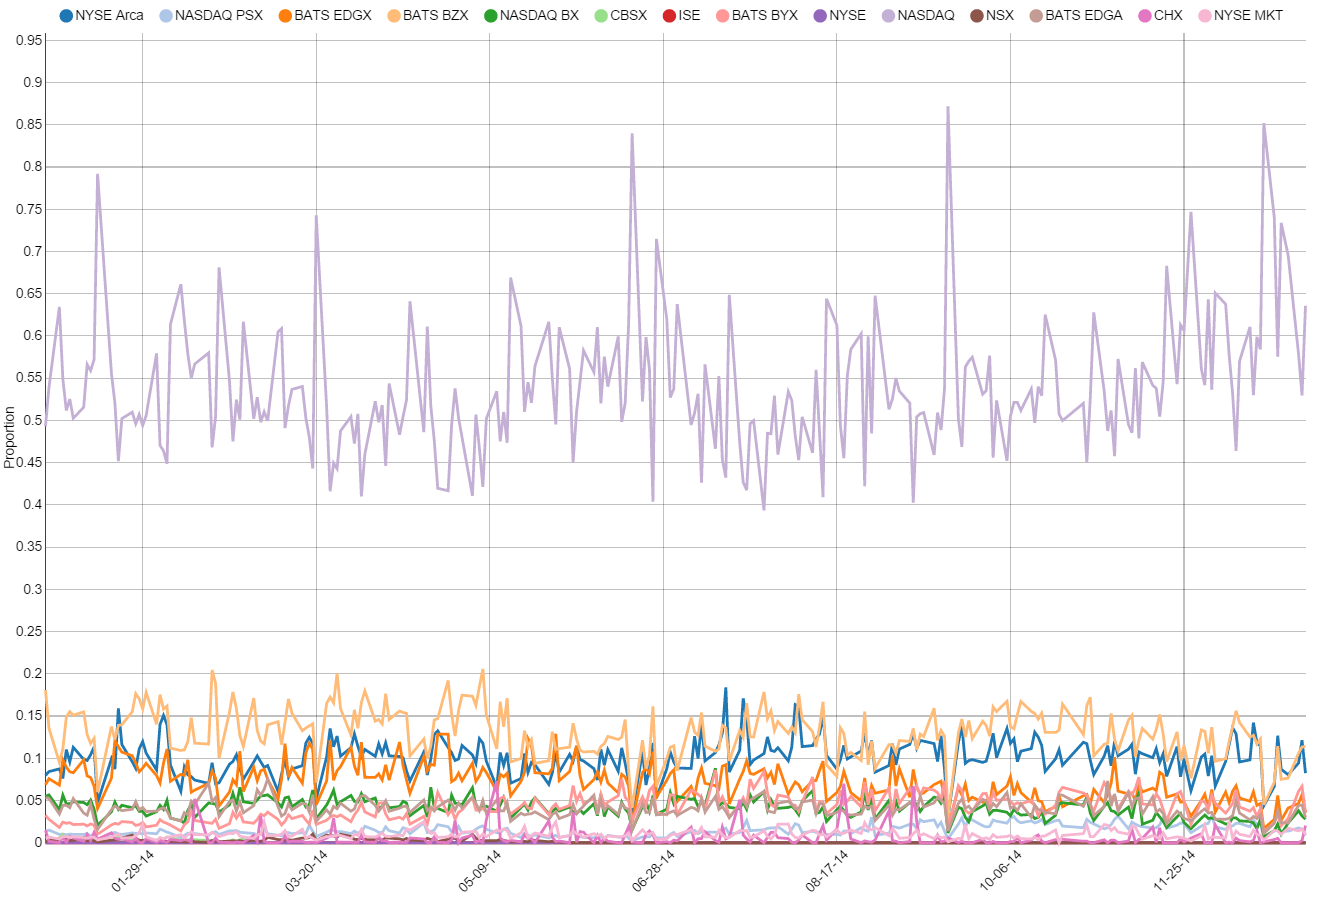
\includegraphics[width=50mm]{{./../output/exchangeShares/linemsft}.png}
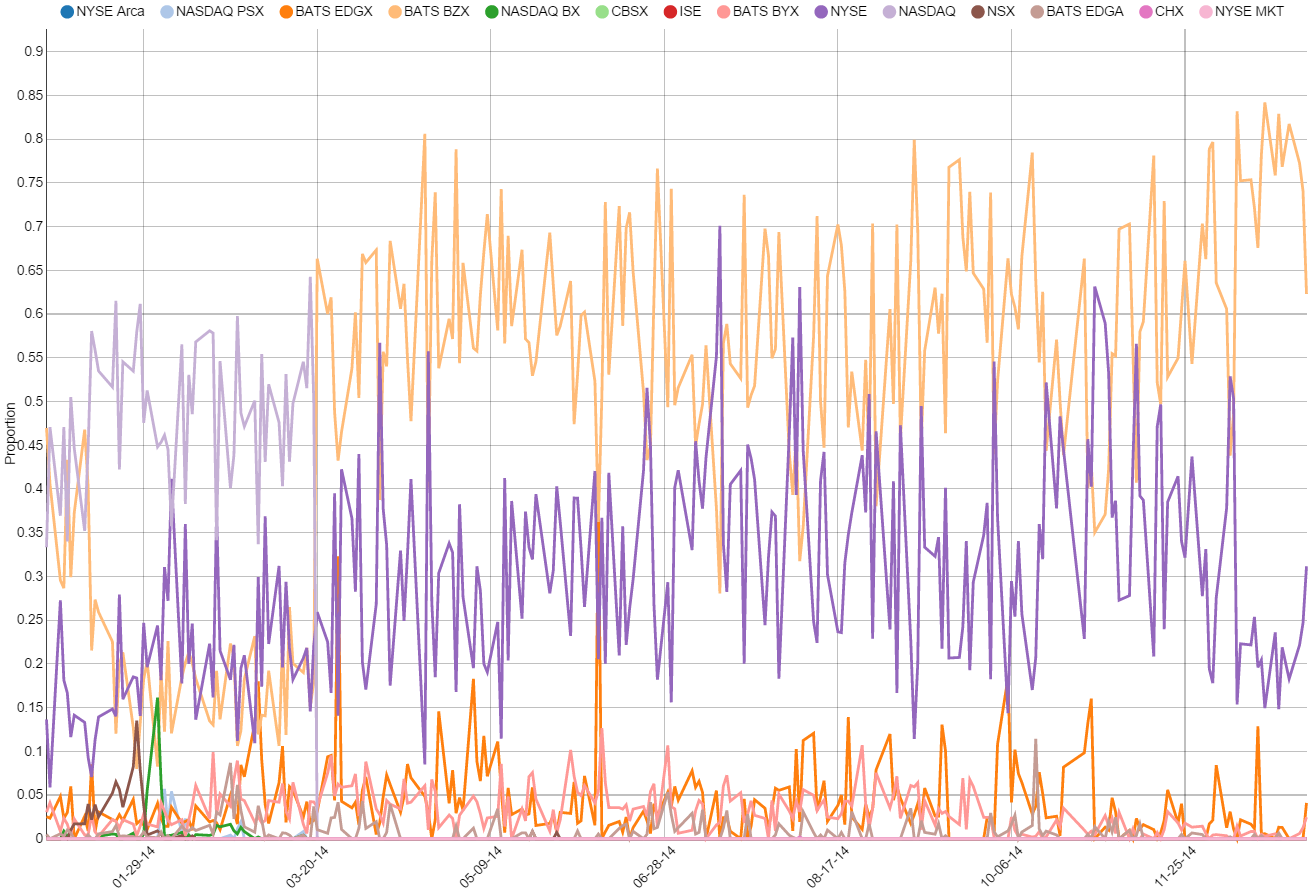
\includegraphics[width=50mm]{{./../output/exchangeShares/linebrka}.png}
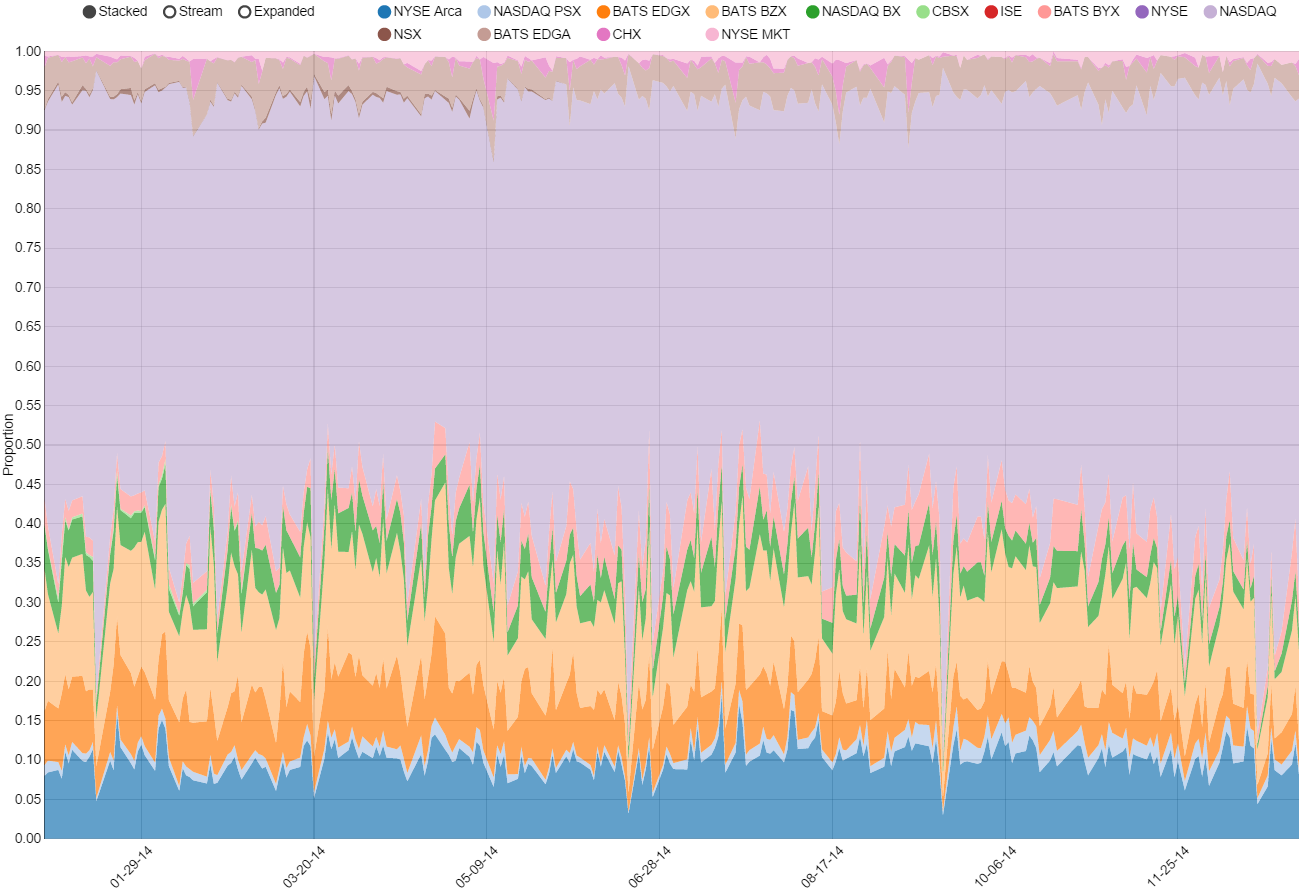
\includegraphics[width=50mm]{{./../output/exchangeShares/stackedAreaMSFT}.png}
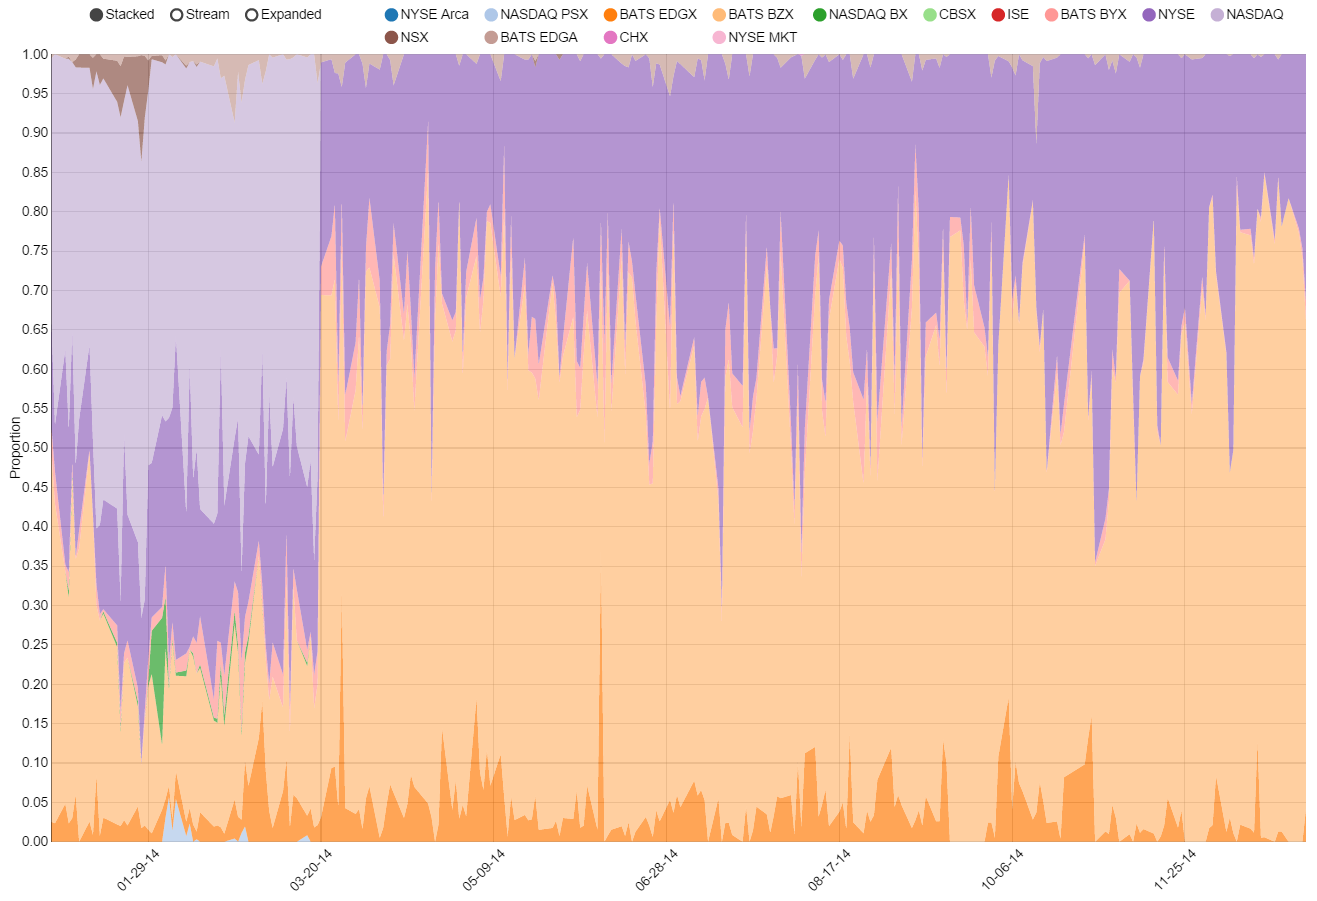
\includegraphics[width=50mm]{{./../output/exchangeShares/stackedAreaBRKA}.png}\\
\caption{The left column shows exchange shares for MSFT in both line and stacked area chart form. The right column shows exchange shares for BRKA.}
\end{figure}
\begin{figure}[H]
\centering
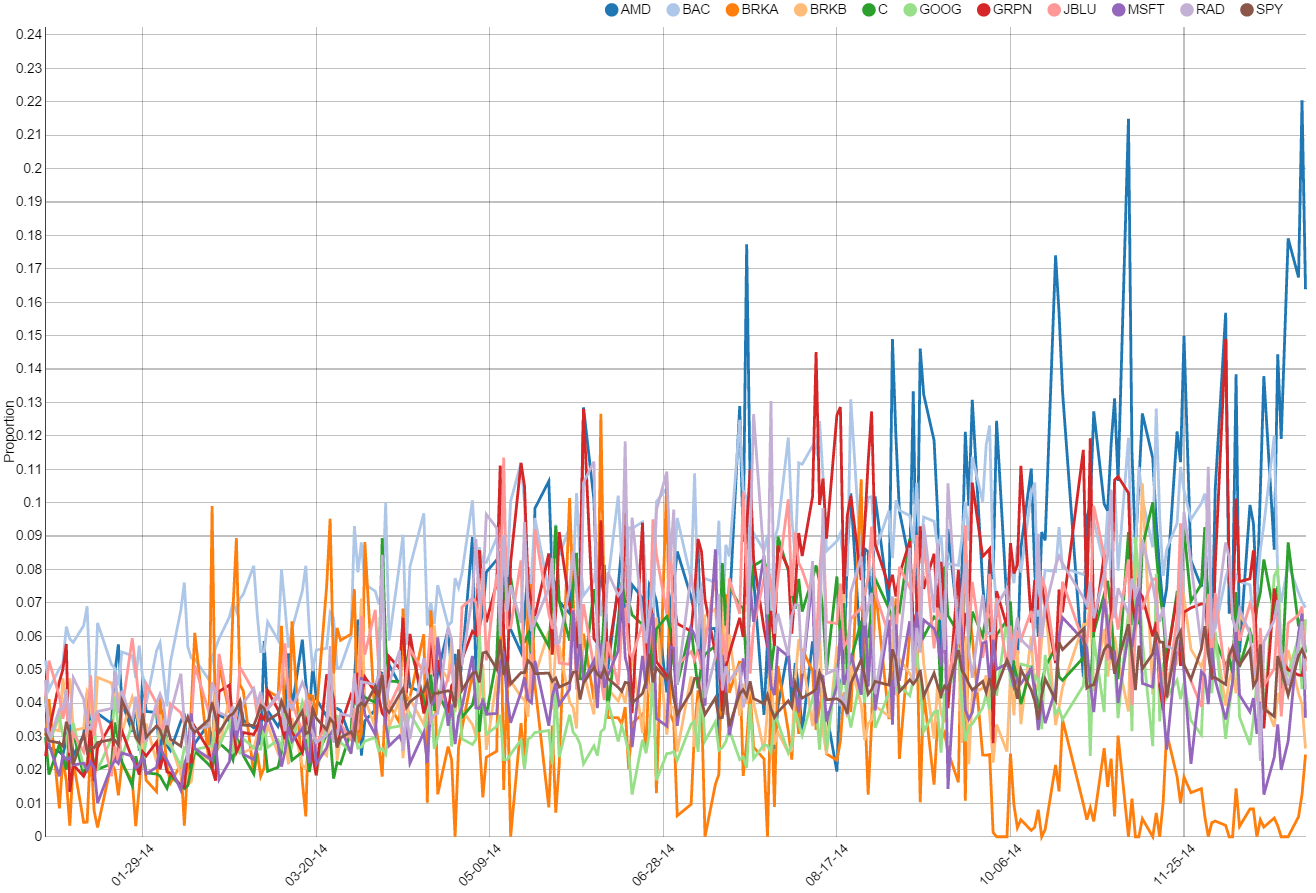
\includegraphics[width=50mm]{{./../output/exchangeShares/linebats.byx}.png}
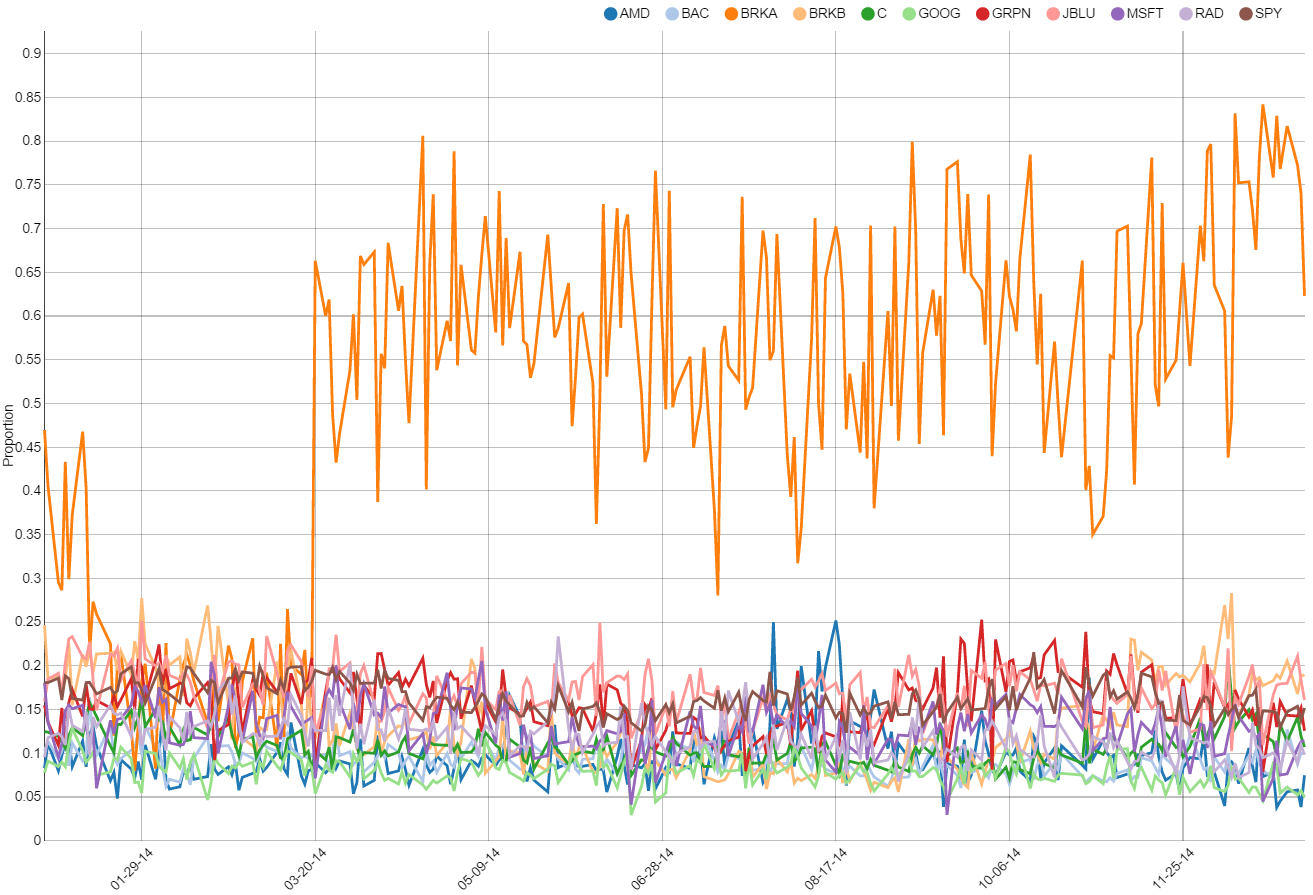
\includegraphics[width=50mm]{{./../output/exchangeShares/linebats.bzx}.png}
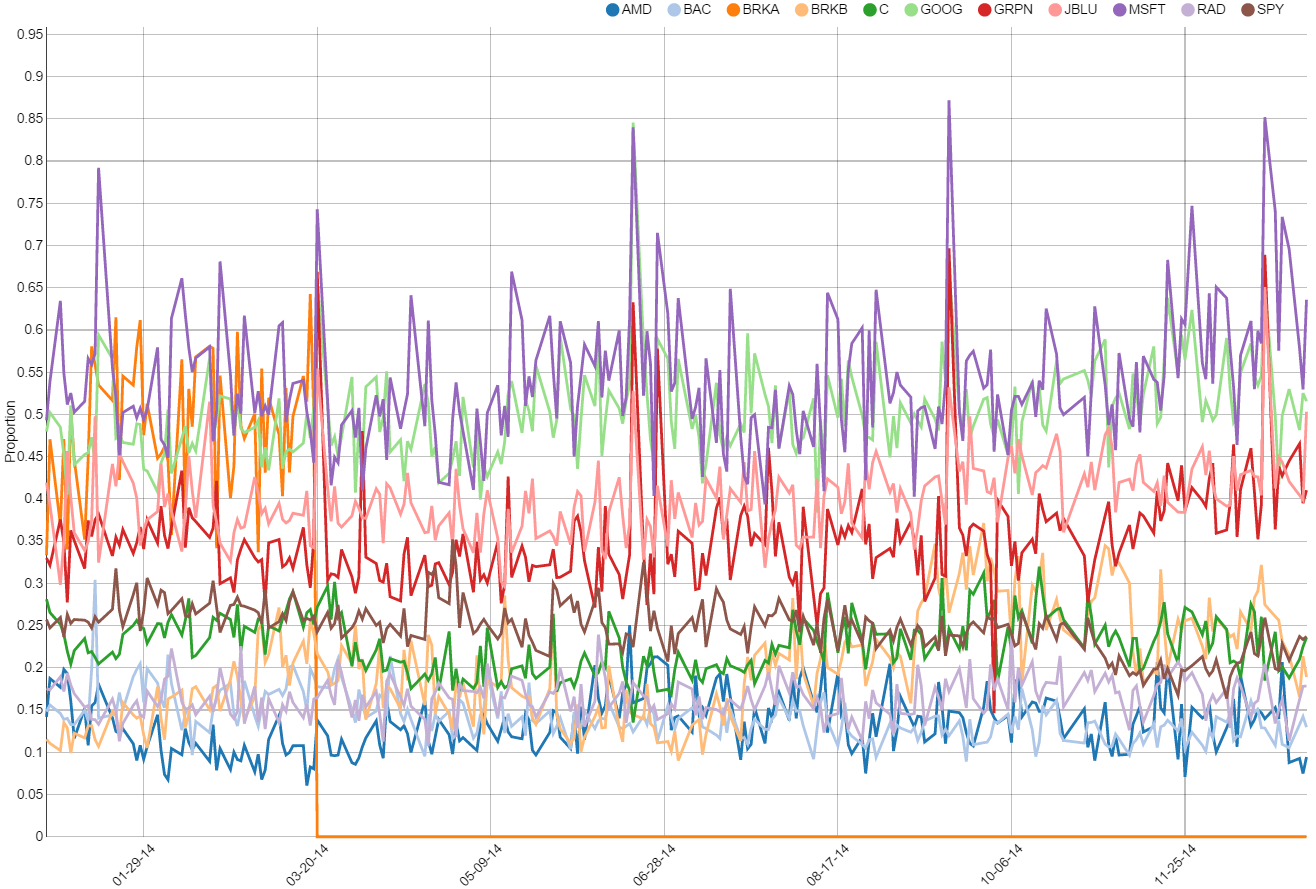
\includegraphics[width=50mm]{{./../output/exchangeShares/linenasdaq}.png}
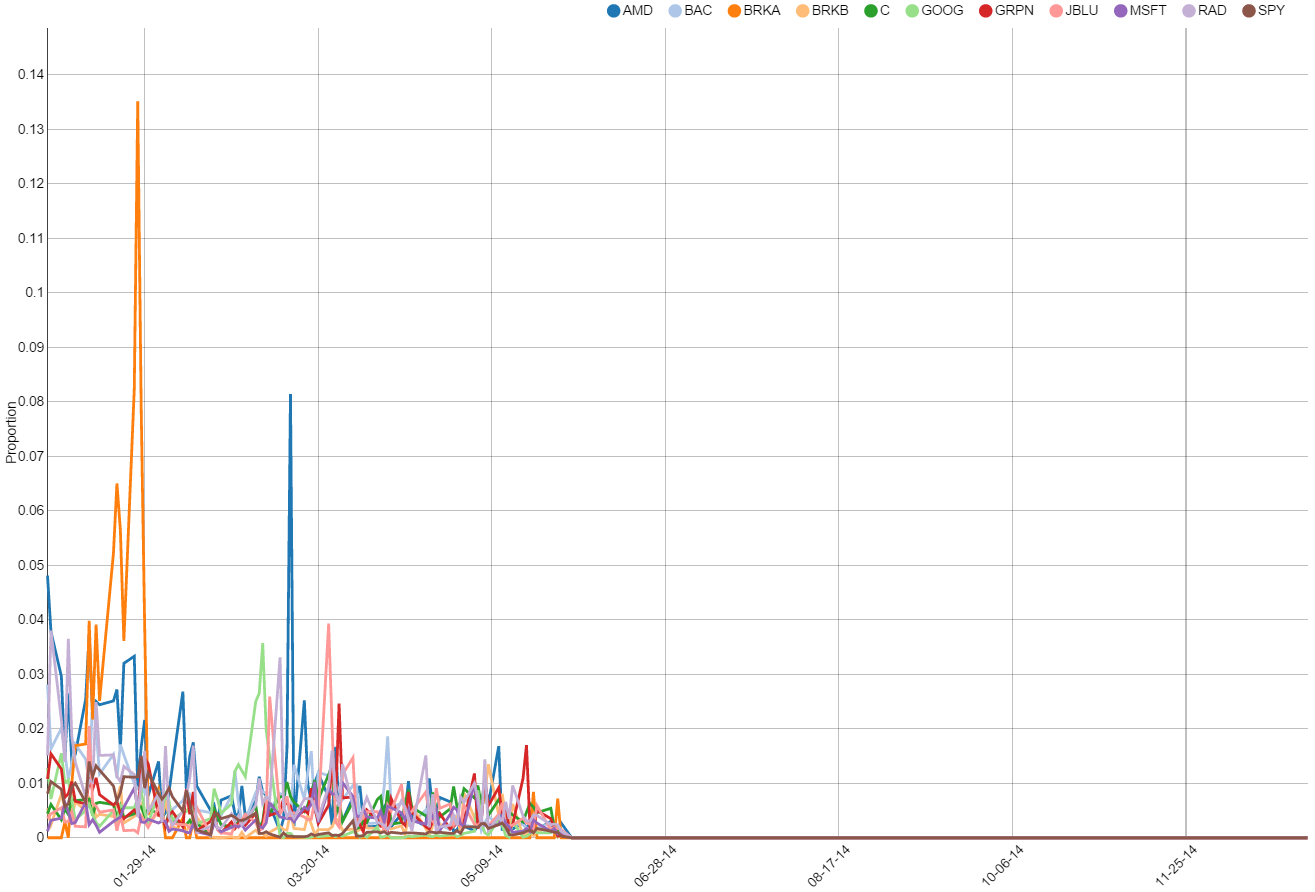
\includegraphics[width=50mm]{{./../output/exchangeShares/linensx}.png}\\
\caption{Each graph shows the daily volumes shares for a given exchange for each of 11 symbols. Clockwise from top left, BATS BYX (shows an increasing trend), BATS BZX (shows BRKA's inflated share due to no recorded NASDAQ volume) , NASDAQ (shows quarterly spikes in some home symbols), and NSX (illustrates its May 2014 demise).}
\end{figure}

\section{Data for Correlation Calculations}
Our data is sourced as above, but covers all trades for a different sample of symbols\footnote{Our sample of symbols consists of AMD, BAC, BRKA, BRKB, C, GOOG, GRPN, JBLU, MSFT, RAD, SPY.} over the period of Jan 1, 2014 - Jan 31, 2014. No time filtering is used, and we are left with 20 trading days total.\\

Future notes: Also explore how market shares look just before close auction, at different times of day, etc. Why do spikes happen in certain exchange. Look at times where we cannot explain, like instituional things. Consider throwing out expiration days, holidays, memorial day weekend.\\		

\section{Partitioning Data}
\subsection{Goals}
From trades data, we wish to get a sense of exchange share over time. In order to transform trades data into exchange share data, we explore two methods of partitioning trades. The exchange shares are computed for each partition of trades.\\

\subsection{Time-Based}
Time is partitioned into windows of equal length, and each trade is assigned to the partition which contains its timestamp. This method allowed for partitions to contain no trades, and we explored three ways to deal with these empty partitions.\\

Within a given symbol, the exchange $j$'s share for the time interval beginning at $T$ is given by
$$s_{jT} = \frac{\sum_{T\underline{<}t < (T+\Delta T)} q_{jt}}{\sum_{T\underline{<}t < (T+\Delta T)}q_{t}}$$
where $q$ refers to a trade's volume and $\Delta T$ refers to the time interval.\\

\subsubsection{Passing Over} \label{passoverempty}
Empty partitions are kept in determining lags, but excluded from contributing to correlation calculations. This is an established R option used via the na.pass argument\footnote{https://stat.ethz.ch/R-manual/R-devel/library/stats/html/acf.html}.\\

\subsubsection{Discarding} \label{discardempty}
Empty partitions are discarded before computing autocorrelations. For example, if partition $t$ and window $t + n$ are separated by $(n - 1)$ empty partitions, they will be considered $t$ and $t + 1$ after discarding the empty partitions.\\

\subsubsection{Persisting Last State Through} \label{persistempty}
To simulate that a regime simply continued if no trading activity occurred, we explored persisting a partition's exchange share through its trailing empty partitions (if they existed). This avenue has been closed, due to its positive biasing of autocorrelation.\\

\subsection{Trade-Based}
Trades are partitioned into sequential groups of $n$ trades. To get a sense of the duration of these partitions, we compute a moving average of these partitions for our dataset.\\

If we index volumes $q$ of trades by $z$, the exchange $j$'s share at interval $k$ is now given by
$$s_{jk} = \frac{\sum_{n \cdot j \underline{<} z < n \cdot (k+1)} q_{jz}}{\sum_{n \cdot k \underline{<} z < n \cdot (k+1)}q_{z}}.$$

\section{Data Transformation}
The main concern about using compositional data is the constraint that all the values sum to 1 in all periods.\\

Further, we wish to normalize an exchange's share based on the exchange's ``typical'' exchange share. To do this, we took the exchange $j$'s share $s$ of stock $i$ in the interval $t$, $s_{ijt}$, and used its deviation from the exchange $j$'s average share $\overline{s}$ of stock $i$ over the available timerange as a proportion of the average share. We call this $z$ and use

$$z_{ijt} = \frac{s_{ijt} - \overline{s_{ij}}}{\overline{s_{ij}}}.$$

\section{Autocorrelation}
\subsection{Goals}
If there exist regimes during which certain exchanges are preferred, then we would exist positive autocorrelations within exchange.\\

\subsection{Comparing Different Partitioning Methods}
Consistently across symbols and intervals, we observe that trade-partitioning yields a clearer decay (and steeper decline) than the time-partitioning methods. Further, the figures reveal that when there is a low rate of empty intervals, the autocorrelation plots are very similar between discarding and passing over empty intervals.\\

As an example, we look to the dataset consisting of AMD trades on BATS EDGX.\\

One interesting thing is the persistence of positive autocorrelations far into the higher-order lags. I suspect this is due to the high number of (0,0) points which bunch up at the lower left corner of Quadrant I. Thus it is very hard for a negative correlation to overcome this ``anchor''. Maybe we should weight points on volume or trade count.

\begin{figure}[H]
\centering
\includegraphics[width=45mm]{{./../output/correlation/AMD/30ClockNaN/acfBATS.EDGX}.png}
\includegraphics[width=45mm]{{./../output/correlation/AMD/30ClockThrowOut/acfBATS.EDGX}.png}
\includegraphics[width=45mm]{{./../output/correlation/AMD/5BusinessNaN/acfBATS.EDGX}.png}
\caption{Autocorrelation plots for BATS EDGX's exchange share: the top two plots used a time-partitioning scheme whereby trades were assigned to windows resulting from partitioning the timerange into 30 second intervals. The left plot passed over empty intervals as described in section \ref{passoverempty}, and the right plot discarded empty intervals as described in section \ref{discardempty}. The third plot used a trade-partitioning scheme whereby trades were partitioned sequentially into groups of 5; note that this yields a more geometric decay and a steeper decline than the preious autocorrelation plots.}
\end{figure}

\section{Inter-Exchange Correlations}
We explore correlations among exchange shares within the same period, and correlations among exchange share across periods separated by a lag.\\

\subsection{Within-Period Correlation} \label{withinperiodcorr}
The following are correlation matrices for various symbols which embody trends representative of the sample.\\

The exchanges are ordered such that the minor exchanges\footnote{NSX, CBSX, NASDAQ.PSX, and CHX.} are grouped at the top-left. They are followed by the Taker/Maker exchanges\footnote{BATS.BYX, BATS.EDGA, and NASDAQ.BX}. The final five exchanges are the Maker/Taker exchanges\footnote{NYSE, NYSE.Arca, BATS.BZX, and NASDAQ.}.\\

The value in cell $(i, j)$ is the correlation of exchange $i$'s share score with exchange $j$'s share score.\\
$$r_{z_iz_j} = \frac{\sum_{t=1}^{n} z_{it} z_{jt} - n\bar{z_i}\bar{z_j}}{(n-1)s_{z_i}s_{z_j}}$$
where $z_{it}$ and $z_{jt}$ are exchange volume share scores for exchange $a$ and $b$ at time $t$, and $s_{z_i}$ and $s_{z_j}$ are the sample standard deviations for $z_{it}$ and $z_{jt}$, respectively.

\begin{figure}[H]
\centering
\includegraphics[width=40mm]{{./../output/correlation/MSFT/20BusinessNaN/correlationMatrixUnLagged}.png}
\includegraphics[width=40mm]{{./../output/correlation/GOOG/20BusinessNaN/correlationMatrixUnLagged}.png}
\includegraphics[width=40mm]{{./../output/correlation/SPY/20BusinessNaN/correlationMatrixUnLagged}.png}
\includegraphics[width=40mm]{{./../output/correlation/GRPN/20BusinessNaN/correlationMatrixUnLagged}.png}
\includegraphics[width=40mm]{{./../output/correlation/BAC/20BusinessNaN/correlationMatrixUnLagged}.png}
\includegraphics[width=40mm]{{./../output/correlation/C/20BusinessNaN/correlationMatrixUnLagged}.png}\\
\caption{Correlation matrices for exchange shares in various stocks, using the trade-partitioning method for 20 trade intervals. Note correlations among the Taker/Maker exchange shares are positive. However, the Maker/Taker exchange shares show negative correlations between each other and against the Taker/Maker exchanges. There is an interesting pattern in BAC where the strongest correlations are those between exchanges of different fee structure; within the two groups of exchanges, correlations are less negative.}
\end{figure}
\begin{figure}[H]
\centering
\includegraphics[width=40mm]{{./../output/correlation/MSFT/60ClockNaN/correlationMatrixUnLagged}.png}
\includegraphics[width=40mm]{{./../output/correlation/GOOG/60ClockNaN/correlationMatrixUnLagged}.png}
\includegraphics[width=40mm]{{./../output/correlation/SPY/60ClockNaN/correlationMatrixUnLagged}.png}
\includegraphics[width=40mm]{{./../output/correlation/GRPN/60ClockNaN/correlationMatrixUnLagged}.png}
\includegraphics[width=40mm]{{./../output/correlation/BAC/60ClockNaN/correlationMatrixUnLagged}.png}
\includegraphics[width=40mm]{{./../output/correlation/C/60ClockNaN/correlationMatrixUnLagged}.png}\\
\caption{Correlation matrices for exchange shares in various stocks, using the time-partitioning method for 60 second intervals (method for dealing with empty intervals does not affect within-period correlations). The same patterns as in the previous set of graphs are present, with the particular correlations among Maker/Taker exchanges particularly dampened.}
\end{figure}

\subsection{Single Lagged Correlation}
The following are correlation matrices for various symbols which embody trends representative of the sample. The exchanges are ordered just as in section \ref{withinperiodcorr}.\\

The value in cell $(i, j)$ is the correlation of exchange $i$'s share with exchange $j$'s share in the next (lag 1) period.\\
$$r_{z_{i}z_{j}} = \frac{\sum_{t=1}^{n-1} z_{it} z_{j(t+1)} - n\bar{z_i}\bar{z_j}}{(n-2)\gamma_{z_i}\gamma_{z_j}}$$
where $z_{i,t}$ and $z_{j,t}$ are exchange volume share scores for exchange $a$ and $b$ at time $t$, and $\gamma_{z_i}$ and $\gamma_{z_j}$ are the sample standard deviations for $z_{it}$ and $z_{jt}$, respectively.

\begin{figure}[H]
\centering
\includegraphics[width=40mm]{{./../output/correlation/MSFT/20BusinessNaN/correlationMatrixLagged}.png}
\includegraphics[width=40mm]{{./../output/correlation/GOOG/20BusinessNaN/correlationMatrixLagged}.png}
\includegraphics[width=40mm]{{./../output/correlation/SPY/20BusinessNaN/correlationMatrixLagged}.png}
\includegraphics[width=40mm]{{./../output/correlation/GRPN/20BusinessNaN/correlationMatrixLagged}.png}
\includegraphics[width=40mm]{{./../output/correlation/BAC/20BusinessNaN/correlationMatrixLagged}.png}
\includegraphics[width=40mm]{{./../output/correlation/C/20BusinessNaN/correlationMatrixLagged}.png}\\
\caption{Correlation matrices for exchange shares in various stocks, using the trade-partitioning method for 20 trade interals. The diagonal is simply the lag 1 autocorrelation for the respective exchange. Though weak, we can see a fainter inter-exchange effect analagous to within-period inter-exchange correlations.}
\end{figure}
\begin{figure}[H]
\centering
\includegraphics[width=40mm]{{./../output/correlation/MSFT/60ClockNaN/correlationMatrixLagged}.png}
\includegraphics[width=40mm]{{./../output/correlation/GOOG/60ClockNaN/correlationMatrixLagged}.png}
\includegraphics[width=40mm]{{./../output/correlation/SPY/60ClockNaN/correlationMatrixLagged}.png}
\includegraphics[width=40mm]{{./../output/correlation/GRPN/60ClockNaN/correlationMatrixLagged}.png}
\includegraphics[width=40mm]{{./../output/correlation/BAC/60ClockNaN/correlationMatrixLagged}.png}
\includegraphics[width=40mm]{{./../output/correlation/C/60ClockNaN/correlationMatrixLagged}.png}\\
\caption{Correlation matrices for exchange shares in various stocks, using the time-partitioning method for 60 second intervals. The weak inter-exchange correlation trends mirror those in previous correlation matrices.}
\end{figure}

\iffalse
\includegraphics[width=90mm]{{./../output/correlation/AMD/5BusinessNaN/acfBATS.EDGX}.png}\\
\includegraphics[width=90mm]{{./../output/correlation/BAC/5BusinessNaN/acfBATS.EDGX}.png}\\
\includegraphics[width=90mm]{{./../output/correlation/BRKA/5BusinessNaN/acfBATS.EDGX}.png}\\
\includegraphics[width=90mm]{{./../output/correlation/BRKB/5BusinessNaN/acfBATS.EDGX}.png}\\
\includegraphics[width=90mm]{{./../output/correlation/C/5BusinessNaN/acfBATS.EDGX}.png}\\
\includegraphics[width=90mm]{{./../output/correlation/GOOG/5BusinessNaN/acfBATS.EDGX}.png}\\
\includegraphics[width=90mm]{{./../output/correlation/GRPN/5BusinessNaN/acfBATS.EDGX}.png}\\
\includegraphics[width=90mm]{{./../output/correlation/JBLU/5BusinessNaN/acfBATS.EDGX}.png}\\
\includegraphics[width=90mm]{{./../output/correlation/MSFT/5BusinessNaN/acfBATS.EDGX}.png}\\
\includegraphics[width=90mm]{{./../output/correlation/RAD/5BusinessNaN/acfBATS.EDGX}.png}\\
\includegraphics[width=90mm]{{./../output/correlation/SPY/5BusinessNaN/acfBATS.EDGX}.png}
\fi

\section{Regression}
We also formulate the binary variable $A_{sxt}$ as the indicator function based on whether stock $s$ had activity on exchange $x$ at interval $t$. We then regress this variable on lagged $A_{sxt}$:\\
$$A_{sxt} = \alpha_{sx} + \beta_1\cdot A_{sx(t-1)} + \beta_2\cdot A_{sx(t-2)} + \beta_2\cdot A_{sx(t-3)} + \beta_2\cdot A_{sx(t-4)} + \beta_2\cdot A_{sx(t-5)} + \epsilon.$$\\

Consider adding in a volume variable, because if big volumes trade, then volume goes up necessarily.\\
We find that the resulting $\beta$s are generally positive with significant $p$-values. The coefficients are plotted for some examples here:\\
\begin{figure}[H]
\centering
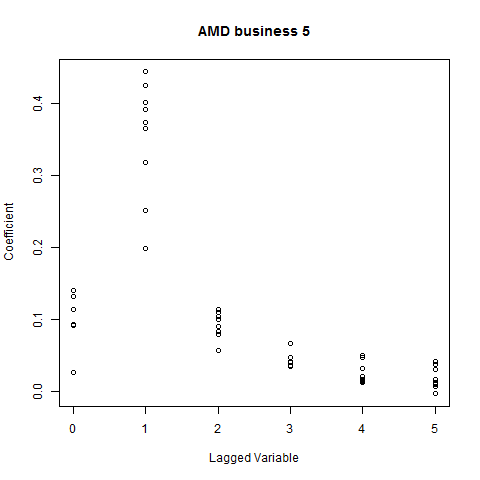
\includegraphics[width=50mm]{{./../output/regression/AMD/businessNaN/5coeffs}.png}
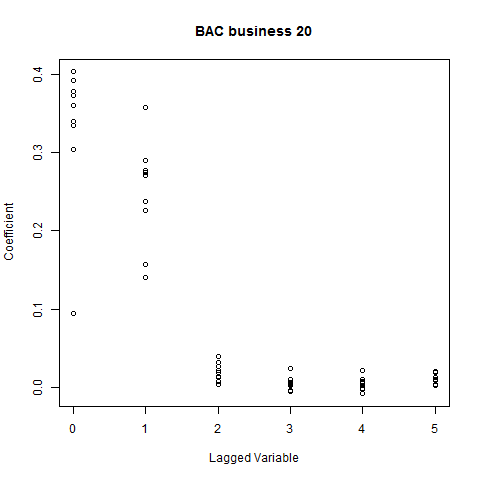
\includegraphics[width=50mm]{{./../output/regression/BAC/businessNaN/20coeffs}.png}
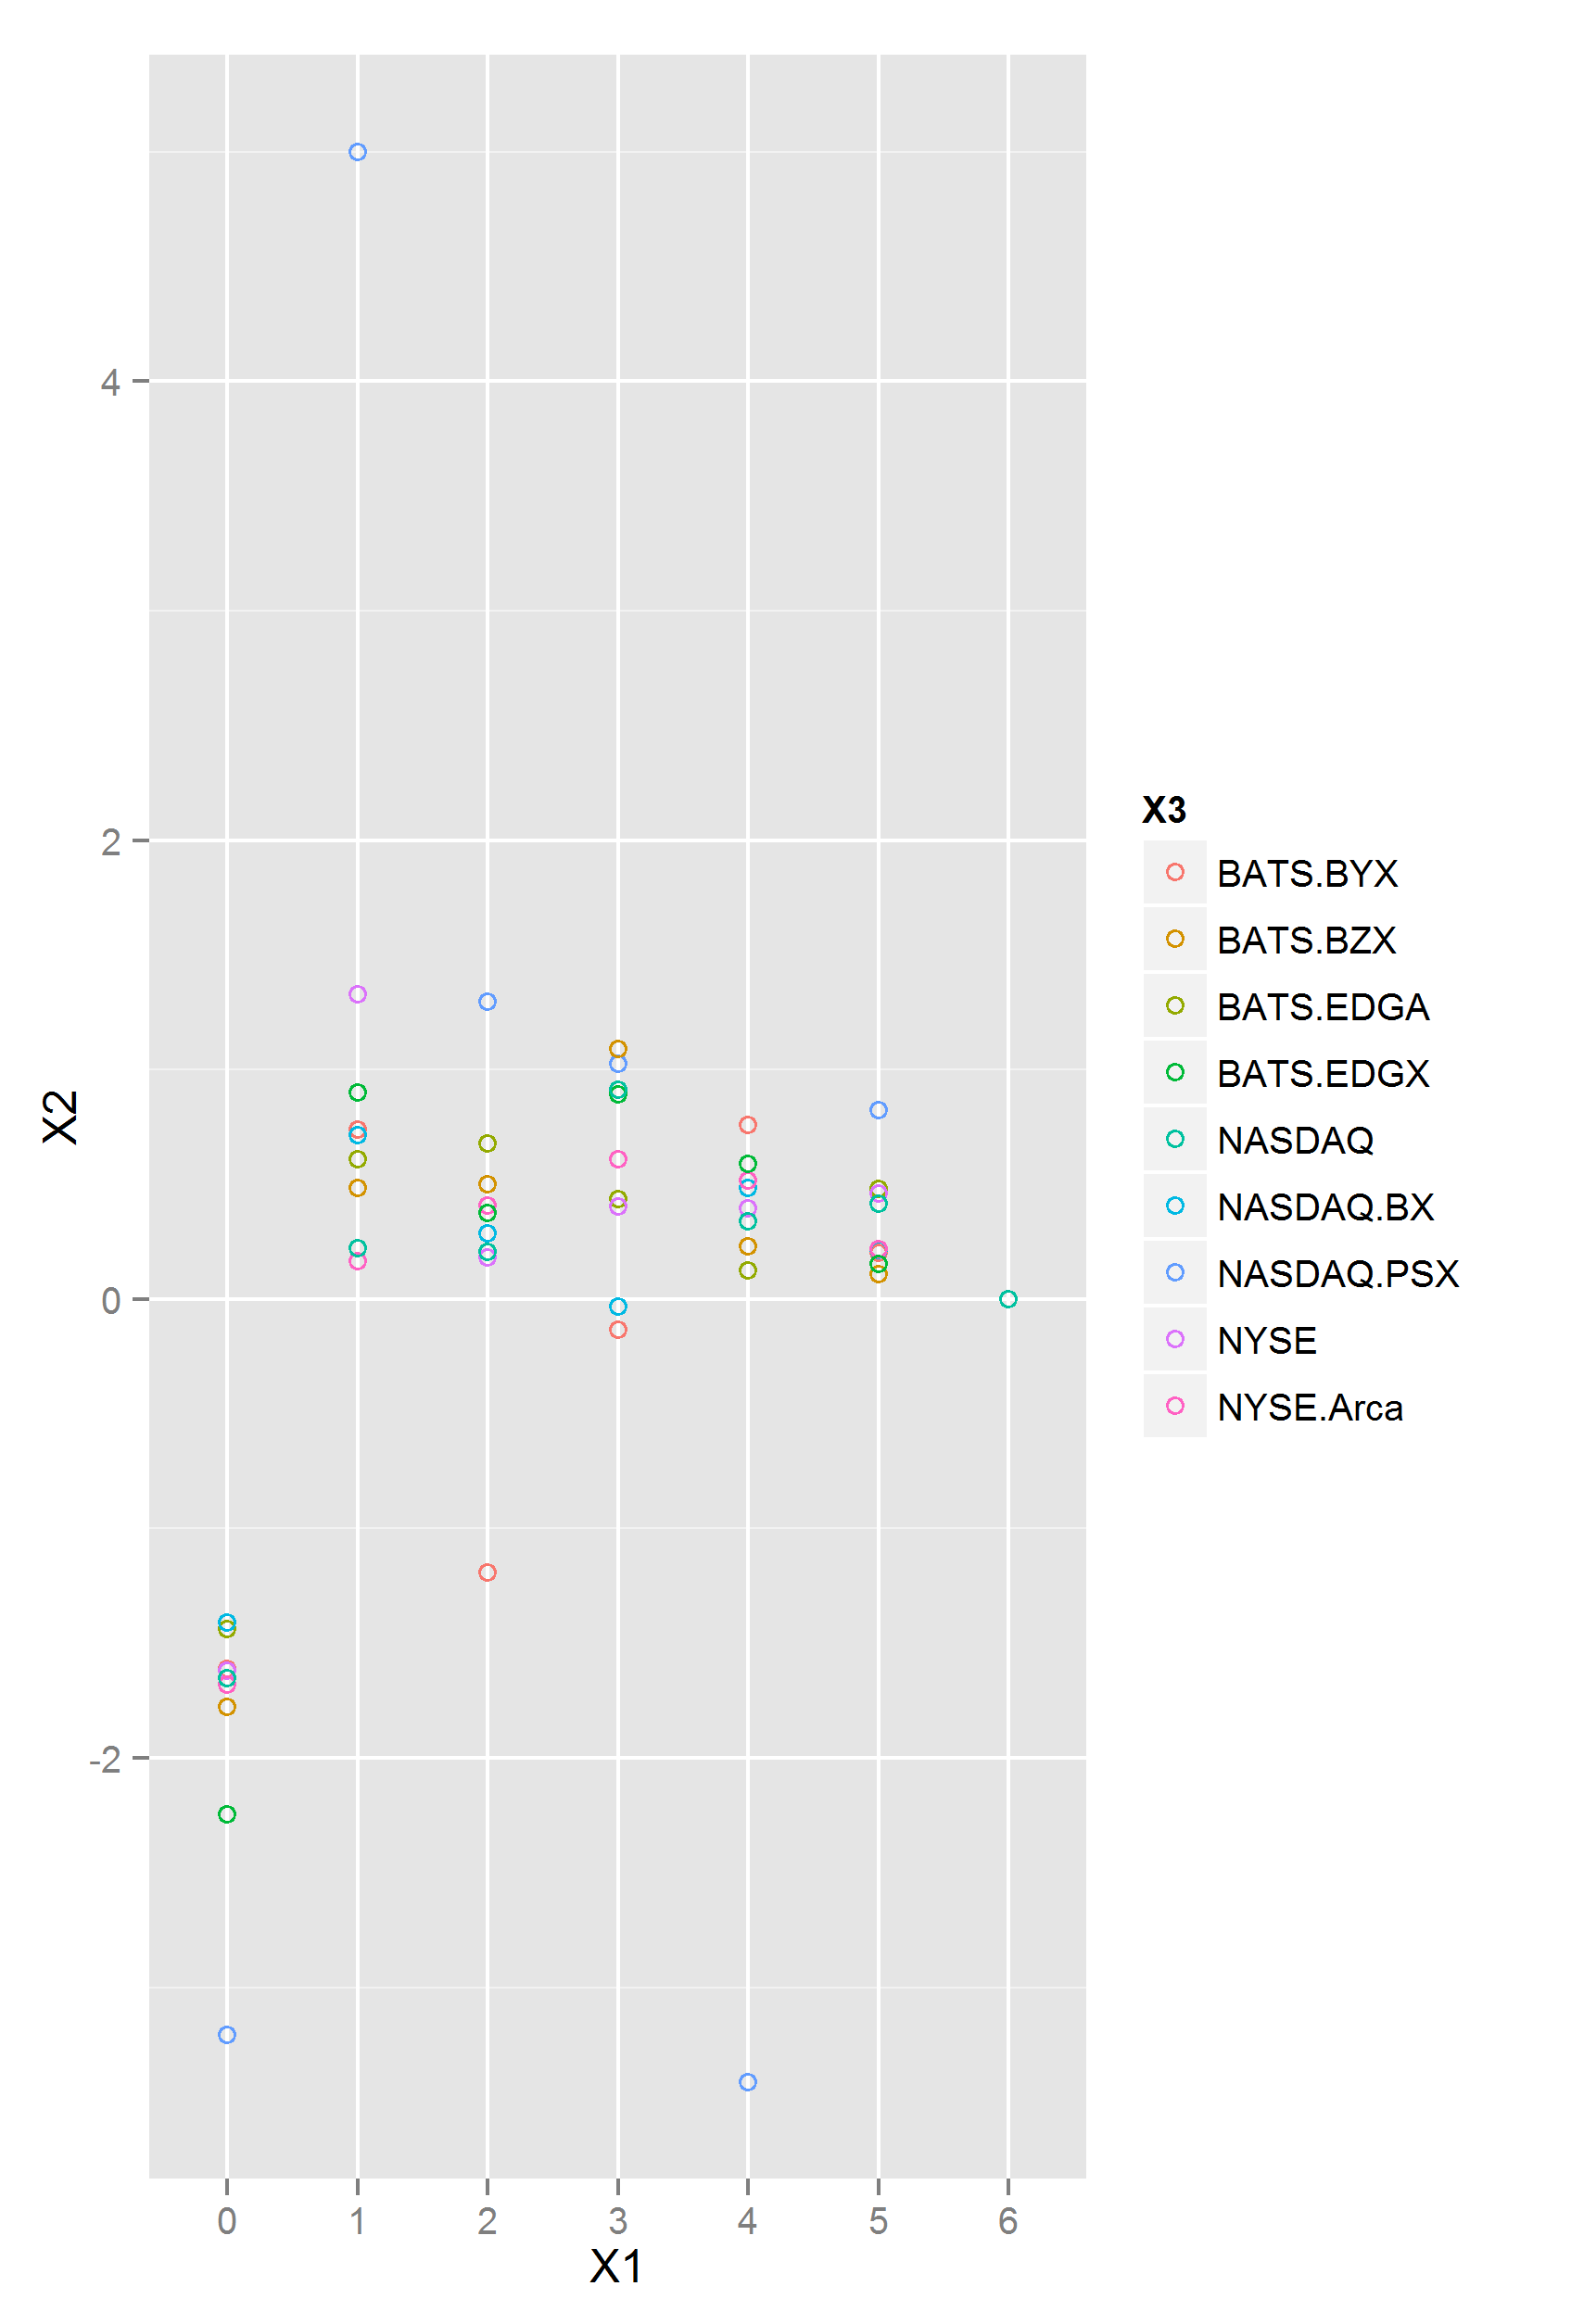
\includegraphics[width=50mm]{{./../output/regression/GOOG/clockNaN/1coeffs}.png}
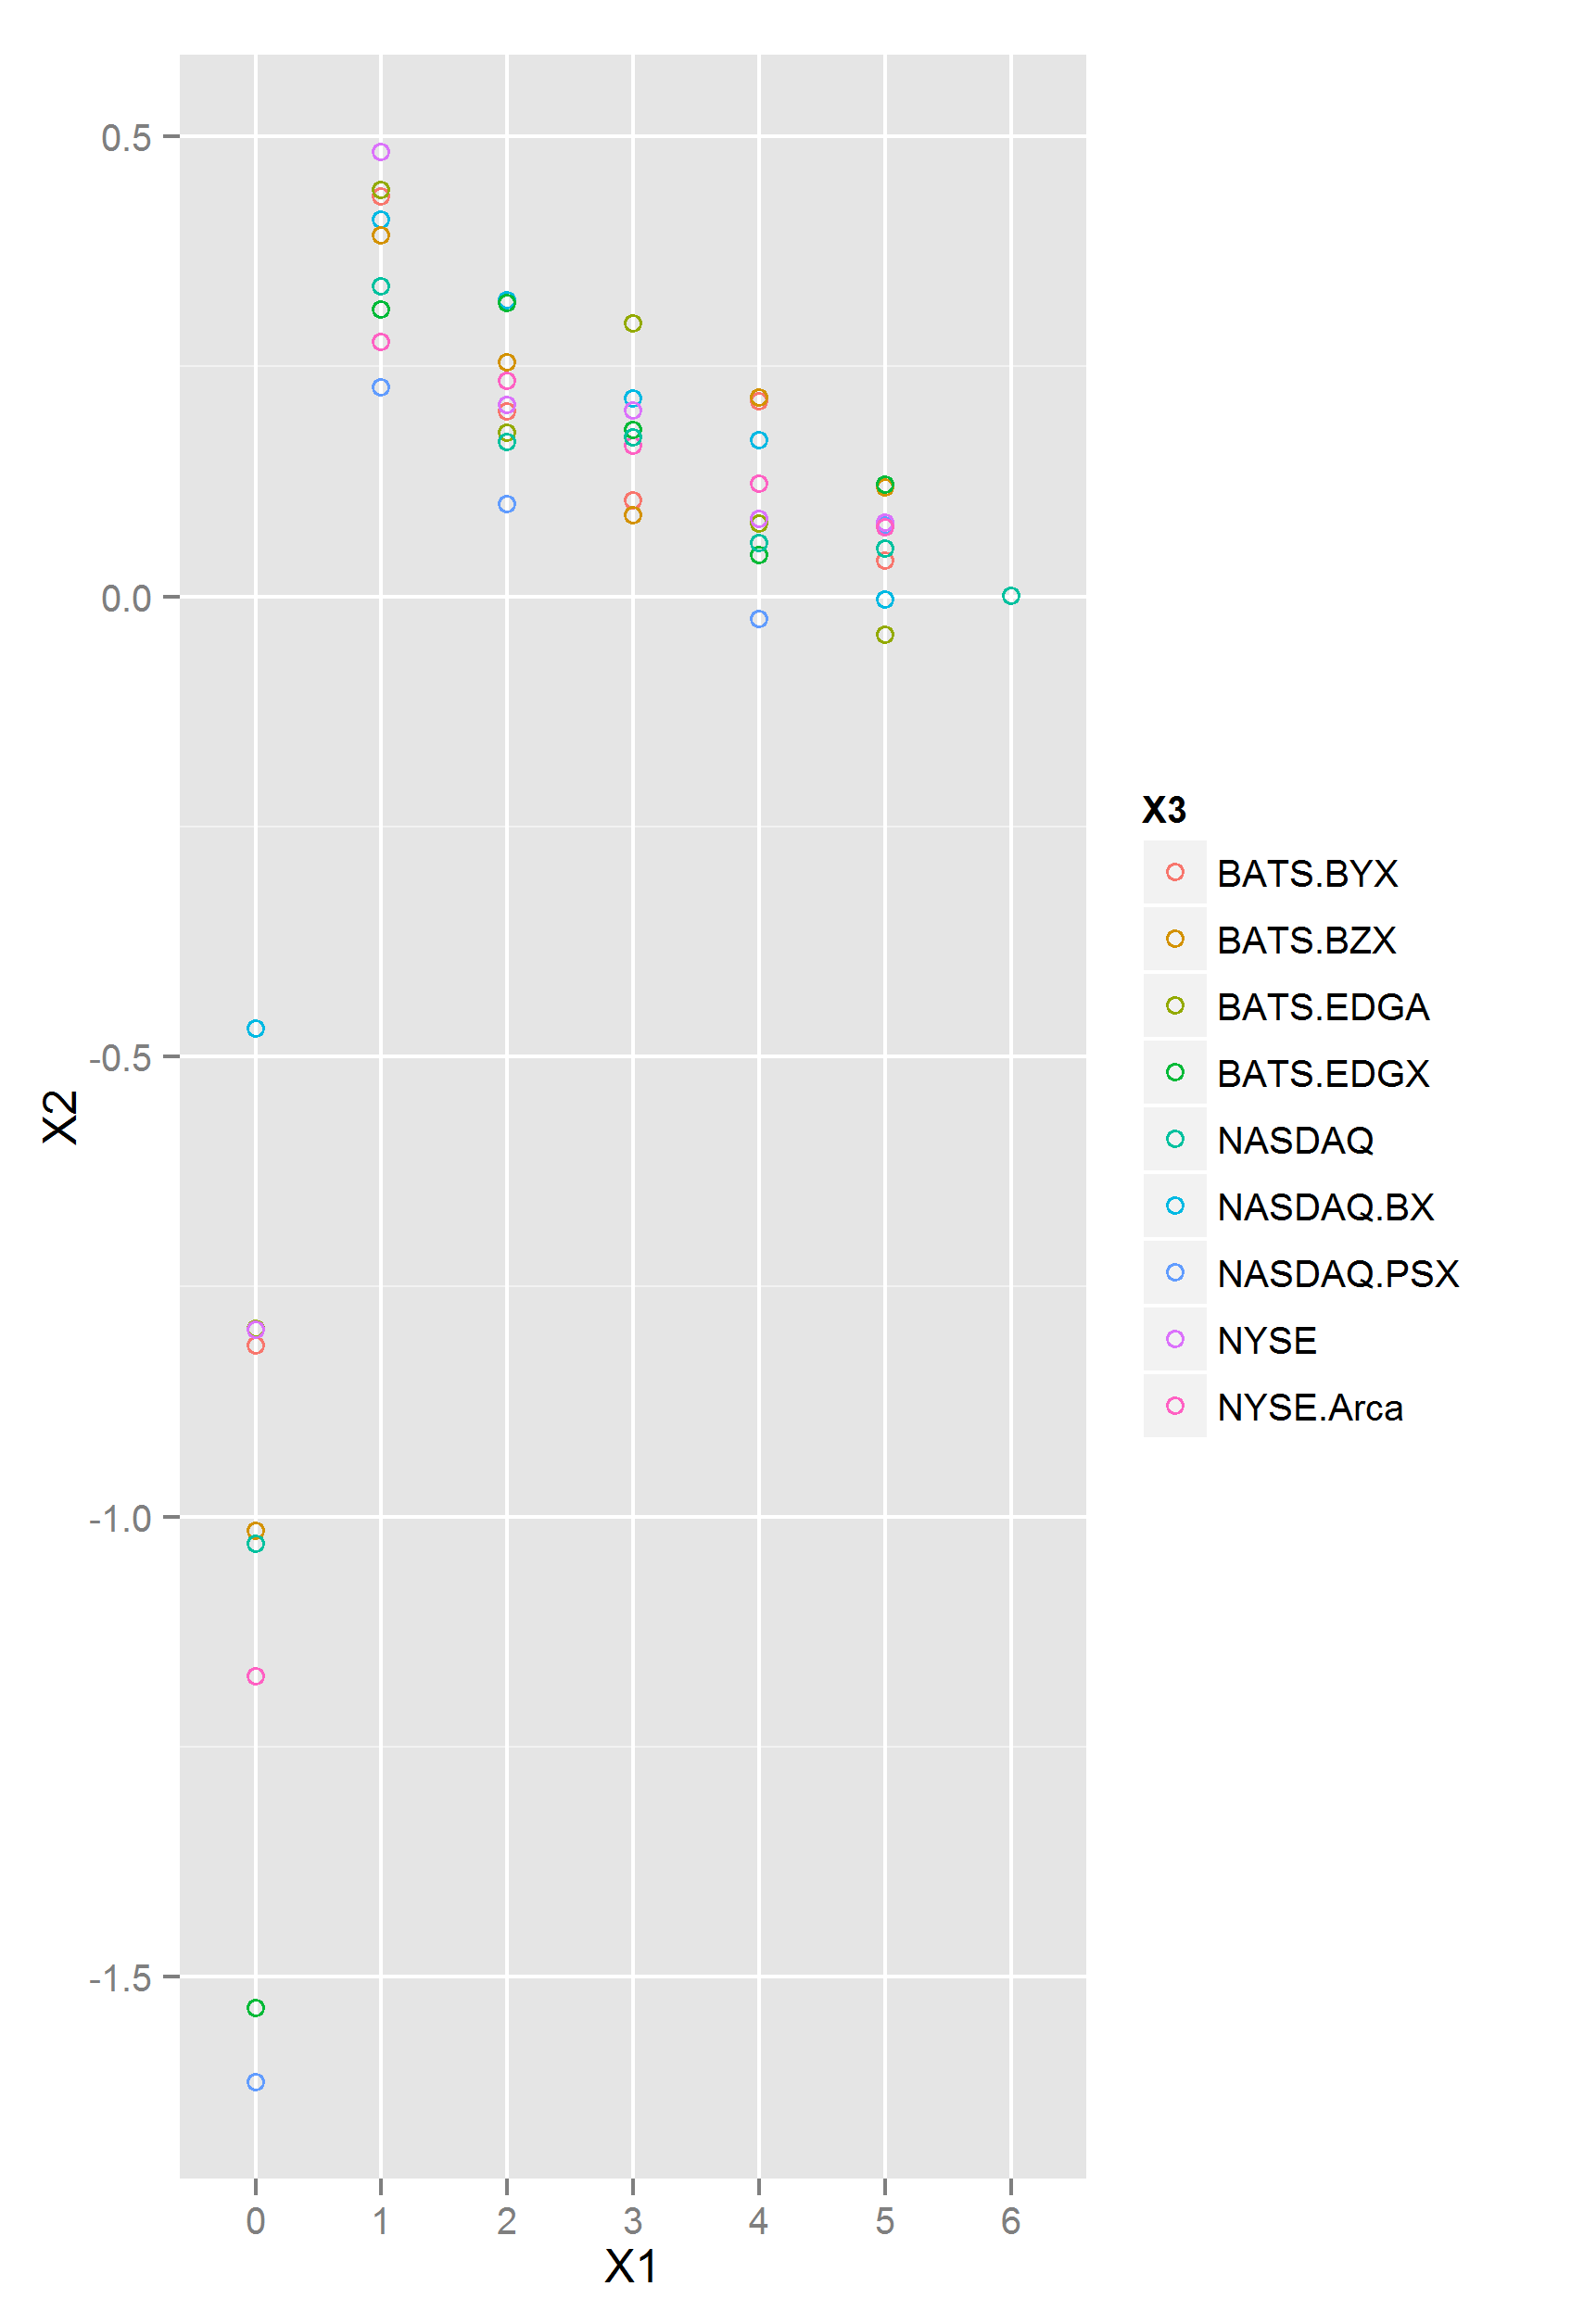
\includegraphics[width=50mm]{{./../output/regression/MSFT/clockNaN/30coeffs}.png}t
\includegraphics[width=50mm]{{./../output/regression/RAD/clockNaN/60coeffs}.png}
\includegraphics[width=50mm]{{./../output/regression/BRKA/clockNaN/60coeffs}.png}\\
\caption{For a given symbol and partitioning method, each graph plots the regression coefficients for the intercept (on $x$=0) and for the lagged variables (on $x \in \{1,2,3,4,5\}$ for each respective lag). As each graph plots for all major exchanges, there is one coefficient for each exchange for each variable.}
\end{figure}

\section{Variance}
Variance of hourly market share, low intraday variance, high interday variance.

\section{Compositional Data}
Statistician Aitchison recommends logratios\footnote{A Concise Guide to Compositional Data Analysis, 2003}.

\end{document}